\documentclass[11pt]{beamer}
\usetheme{CambridgeUS}
\usepackage[utf8]{inputenc}
\usepackage[spanish]{babel}
\usepackage{amsmath}
\usepackage{amsfonts}
\usepackage{amssymb}
\author{Equipo 1}
\title{Integral de Riemann-Stieltjes}
%\setbeamercovered{transparent}
%\setbeamertemplate{navigation symbols}{}
%\logo{}
\institute{Facultad de Matemáticas UV}
%\date{}
%\subject{}
\begin{document}

\begin{frame}
\titlepage
\end{frame}

% \begin{frame}
% \tableofcontents
% \end{frame}

\begin{frame}{Particiones}

\begin{definition}
Sea $[a, b]$ intervalo. Una \textit{partición} de $[a, b]$ es un conjunto de puntos $x_0, x_1,..., x_n$ tales que
\begin{equation*}
	a = x_0 \leq x_1 \leq \dots \leq x_n = b
\end{equation*}
Sean
\begin{equation*}
	\Delta x_i = x_i - x_{i-1} (i = 1, \dots, n)
\end{equation*}
\end{definition}[1]

\begin{center}
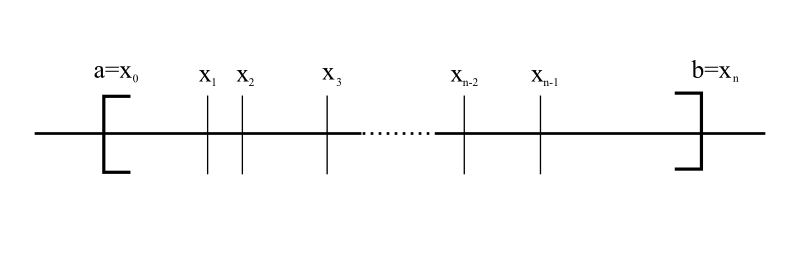
\includegraphics[scale=1]{img/particion.png}
\end{center}

\end{frame}

\begin{frame}{Integral de Riemann}

\begin{definition}[2]
Sea $f$ es una función real acotada definida en $[a, b]$. Para cada partición $P$ de $[a, b]$ definimos

\begin{equation*}
	\begin{array}{rcll}
		M_i & = & \sup f(x) & (x_{i-1} \leq x \leq x_i), \\
		m_i & = & \inf f(x) & (x_{i-1} \leq x \leq x_i), \\
		U(P, f) & = & \sum_{i=1}^n M_i \Delta x_i , \\
		L(P, f) & = & \sum_{i=1}^n m_i \Delta x_i
	\end{array}
\end{equation*}
y finalmente
\begin{equation}
	\begin{array}{rcl}
		\overline{\int}_a^b f\,dx & = & \inf U(P, f)
	\end{array}
\end{equation}
\begin{equation}
	\begin{array}{rcl}
		\underline{\int}_a^b f\,dx & = & \sup L(P, f)
	\end{array}
\end{equation}

Las partes izquierdas de estas ecuaciones son llamadas \textit{integral superior} e \textit{integral inferior} de $f$ sobre $[a, b]$ respectivamente.
\end{definition}

\end{frame}

\begin{frame}{Integral de Riemann}

\begin{definition}[3]
Si las integrales \textit{superior} e \textit{inferior} son iguales entonces decimos que $f$ es \textit{riemann-integrable} en $[a, b]$ y diremos que $f\in \mathcal{R}$ donde $\mathcal{R}$ denota el conjunto de funciones \textit{riemann-integrables} y denotaremos el valor de (1) y (2) como

\begin{equation}
	\int_a^b f(x)\,dx
\end{equation}

A lo cual llamaremos \textit{integral de riemman de $f(x)$}.
\end{definition}

\end{frame}

\begin{frame}{Integral de Riemann-Stieltjes}

Sea $\alpha$ una función monótona creciente definida en $[a, b]$ (y por tanto, acotada). Para cada partición $P$ escribimos

\[
	\Delta \alpha_i = \alpha(x_i) - \alpha(x_{i-1}) \qquad \Delta\alpha_i \geq 0
\]

Para cualquier función acotada en $[a, b]$ definimos

\[
	\begin{array}{rcl}
		U(P, f, \alpha) & = & \sum_{i=1}^n M_i \Delta \alpha_i, \\
		L(P, f, \alpha) & = & \sum_{i=1}^n m_i \Delta \alpha_i,
	\end{array}
\]

Done $M_i$ y $m_i$ son lo mismo que en la definición (2) y finalmente 

\begin{equation}
	\overline{\int}_a^b f\,d\alpha = \inf U(P, f, \alpha),
\end{equation}

\begin{equation}
	\underline{\int}_a^b f\,d\alpha = \sup L(P, f, \alpha),
\end{equation}

\end{frame}

\begin{frame}{Integral de Riemann-Stieltjes}

\begin{definition}[4]

Si los términos de (4) y (5) son iguales, denotaremos su valor común como

\begin{equation}
	\int_a^b f\,d\alpha
\end{equation}

ó

\begin{equation}
	\int_a^b f(x)\,d\alpha(x).
\end{equation}

Que es la \textit{integral de rieman-stieltjes} de $f$ respecto de $\alpha$ sobre $[a, b]$.

Si (6) existe, es decir (5) y (6) son iguales, decimos que $f$ es integrable respecto a $\alpha$ y escribimos $f \in \mathcal{R}(\alpha)$.

\end{definition}

\end{frame}

\begin{frame}{Integral de Riemann-Stieltjes}

\begin{definition}[5]
Decimos que la partición $P^*$ es un \textit{refinamiento} de $P$ si $P^* \supset P$. Dadas dos particiones $P_1$ y $P_2$ decimos que $P^*$ es su \textit{refinamiento común} si $P^* = P_1 \cup P_2$
\end{definition}

\begin{theorem}[1]
Si $P^*$ es un refinamiento de $P$, entonces

\begin{equation}
	L(P, f, \alpha) \leq L(P^*, f, \alpha)
\end{equation}
y
\begin{equation}
	U(P^*, f, \alpha) \leq U(P, f, \alpha)
\end{equation}
\end{theorem}

\end{frame}

\begin{frame}{Teoremas}

\begin{theorem}[2]
\[
	\underline{\int}_a^b f\,d\alpha \leq \overline{\int}_a^b f\,d\alpha
\]
\end{theorem}

\begin{theorem}[3]
$f \in \mathcal{R}(\alpha)$ sobre $[a, b]$ si y sólo si para cada $\epsilon > 0$ existe una partición $P$ tal que
\begin{equation}
	U(P, f, \alpha) - L(P, f, \alpha) < \epsilon
\end{equation}
\end{theorem}

\end{frame}

\begin{frame}{Teoremas}

\begin{theorem}[4]
	\begin{enumerate}
		\item Si se cumple (10) Para alguna $P$ y alguna $\epsilon$, entonces (10) se cumple para cada refinamiento de $P$.
		\item Si (10) se cumple para $P = {x_0, \dots, x_n}$ y si $s_i$ y $t_i$ son puntos arbitrarios en $[x_{i-1}, x_i]$, entonces
		\[
			\sum_{i=1}^n |f(s_i) - f(t_i)|\Delta\alpha_i < \epsilon
		\]
	\end{enumerate}
\end{theorem}

\begin{theorem}[5]
Si $f$ es continua en $[a, b]$ entonces $f \in \mathcal{R}(\alpha)$ sobre $[a, b]$.
\end{theorem}

\end{frame}

\begin{frame}{Teoremas}

\begin{theorem}[6]
Si $f$ es monótona en $[a, b]$, y $\alpha$ es continua en $[a, b]$, entonces $f \in \mathcal{R}(\alpha)$
\end{theorem}

\begin{theorem}[7]
Supóngase que $f$ es acotada y tiene un número finito de discontinuidades en $[a, b]$, y suponga que $\alpha$ es continua en cada punto en que $f$ es discontinua. Entonces $f \in \mathcal{R}(\alpha)$
\end{theorem}

\begin{theorem}[8]
Suponga que $f \in \mathcal{R}(\alpha)$ en $[a, b]$, $m \leq f \leq M$, $\phi$ es continua en $[m, M]$ y $h(x) = \phi(f(x))$ en $[a, b]$. Entonces $h \in \mathcal{R}(\alpha)$ en $[a, b]$
\end{theorem}

\end{frame}

\begin{frame}[allowframebreaks]{Propiedades de la integral}
\begin{enumerate}
	\item Si $f_1, f_2 \in \mathcal{R}(\alpha)$ en $[a, b]$ entonces
	\[
		f_1 + f_2 \in \mathcal{R}(\alpha),
	\]
	$cf \in \mathcal{R}(\alpha)$ para cualquier constante $c$, y
	\[
		\begin{array}{rcl}
			\int_a^b (f_1 + f_2) d\alpha & = & \int_a^b f_1 d\alpha + \int_a^b f_2 d\alpha,\\
			\int_a^b cf\,d\alpha & = & c \int_a^b f\,d\alpha.
		\end{array}
	\]
	\item Si $f_1(x) \leq f_2(x)$ en $[a, b]$ entonces
	\[
		\int_a^b f_1\,d\alpha \leq \int_a^b f_2\,d\alpha
	\]
	\item Si $f \in \mathcal{R}(\alpha)$ en $[a, b]$ y $a < c < b$, entonces $f \in \mathcal{R}(\alpha)$ en $[a, c]$ y en $[c, b]$ y
	\[
		\int_a^c f\,d\alpha + \int_c^b f\,d\alpha = \int_a^b f\,d\alpha
	\]
	\item Si $f \in \mathcal{R}(\alpha)$ y $|f(x)| \leq M$ en $[a, b]$ entonces
	\[
		|\int_a^b f\,d\alpha| \leq M[\alpha(b) - \alpha(a)]
	\]
	\item Si $f \in \mathcal{R}(\alpha_1)$ y $f \in \mathcal{R}(\alpha_2)$, entonces $f \in \mathcal{R}(\alpha_1 + \alpha_2)$ y
	\[
		\int_a^b f\,d(\alpha_1 + \alpha_2) = \int_a^b f\,d\alpha_1 + \int_a^b f\,d\alpha_2 ;
	\]
	si $f \in \mathcal{R}(\alpha)$ y $c$ es una constante positiva, entonces $f \in \mathcal{R}(c\alpha)$ y
	\[
		\int_a^b f\,d(c\alpha) = c \int_a^b f\,d\alpha.
	\]
\end{enumerate}
\end{frame}

\end{document}

